\documentclass[10pt,a4paper]{article}

\usepackage[a4paper, top=0.9cm, bottom=0.9cm, left=1cm, right=1cm]{geometry}
\usepackage{graphicx}
\usepackage{float}
\usepackage{amsmath}
\usepackage{amssymb}
\usepackage{xcolor}
\usepackage{mdframed}
\usepackage{parskip}
\usepackage{enumitem}
\usepackage{titlesec}
\usepackage{booktabs}
\usepackage{array}
\usepackage{tikz}
\usetikzlibrary{arrows.meta, positioning}
\usepackage[T1]{fontenc}

\graphicspath{{../../reference/Network_extracted/figures/Lecture6/}}

\definecolor{keyblue}{RGB}{30, 80, 160}
\definecolor{keybluebg}{RGB}{220, 235, 255}
\definecolor{noteorange}{RGB}{200, 100, 0}
\definecolor{noteorangebg}{RGB}{255, 240, 215}
\definecolor{warnred}{RGB}{180, 30, 30}
\definecolor{warnredbg}{RGB}{255, 220, 220}
\definecolor{defgreen}{RGB}{20, 110, 50}
\definecolor{defgreenbg}{RGB}{215, 245, 225}
\definecolor{headernavy}{RGB}{25, 35, 90}

\newmdenv[linecolor=keyblue,backgroundcolor=keybluebg,linewidth=1.5pt,
  leftline=true,rightline=false,topline=false,bottomline=false,
  innerleftmargin=7pt,innerrightmargin=6pt,
  innertopmargin=3pt,innerbottommargin=3pt,
  skipabove=3pt,skipbelow=3pt]{keybox}

\newmdenv[linecolor=noteorange,backgroundcolor=noteorangebg,linewidth=1.5pt,
  leftline=true,rightline=false,topline=false,bottomline=false,
  innerleftmargin=7pt,innerrightmargin=6pt,
  innertopmargin=3pt,innerbottommargin=3pt,
  skipabove=3pt,skipbelow=3pt]{notebox}

\newmdenv[linecolor=defgreen,backgroundcolor=defgreenbg,linewidth=1.5pt,
  leftline=true,rightline=false,topline=false,bottomline=false,
  innerleftmargin=7pt,innerrightmargin=6pt,
  innertopmargin=3pt,innerbottommargin=3pt,
  skipabove=3pt,skipbelow=3pt]{defbox}

\newmdenv[linecolor=warnred,backgroundcolor=warnredbg,linewidth=1.5pt,
  leftline=true,rightline=false,topline=false,bottomline=false,
  innerleftmargin=7pt,innerrightmargin=6pt,
  innertopmargin=3pt,innerbottommargin=3pt,
  skipabove=3pt,skipbelow=3pt]{warnbox}

\titleformat{\section}[block]{\normalsize\bfseries\color{headernavy}}{}{0pt}{}
  [\vspace{1pt}\rule{\linewidth}{0.6pt}\vspace{2pt}]
\titleformat{\subsection}[block]{\small\bfseries\color{keyblue}}{}{0pt}{}
\titlespacing*{\section}{0pt}{5pt}{2pt}
\titlespacing*{\subsection}{0pt}{3pt}{1pt}

\setlist{nosep, topsep=1pt, itemsep=1pt, leftmargin=1.3em}
\parskip=2pt
\parindent=0pt

% ===========================================================================
\begin{document}
% ===========================================================================

\begin{center}
  {\large\bfseries\color{headernavy} Q5 \textemdash{} End-to-End Performance Using TCP}\\[1pt]
  {\small MM6 $\cdot$ Hans-Peter Schwefel}
\end{center}
\vspace{1pt}\hrule height 1pt\vspace{4pt}
TCP has multiple built-in \textbf{mechanisms} to ensure reliable and fair data transfer over a shared network:
\begin{itemize}
  \item \textbf{Handshake:} establishes the connection before data flows --- ensures both ends are ready and agrees on initial sequence numbers.
  \item \textbf{Flow control:} receiver advertises how much buffer space it has --- prevents the sender from overwhelming the receiver.
  \item \textbf{Congestion control:} sender adapts its sending rate based on network feedback --- prevents the sender from overwhelming the \emph{network}.
\end{itemize}

We focus on \textbf{congestion control} --- how TCP detects and reacts to congestion, walk through a concrete scenario, and introduce a Markov chain model to capture TCP's behaviour analytically.


\vspace{3pt}


% ===========================================================================
\section*{1\quad TCP Congestion Control}
% ===========================================================================
TCP congestion control regulates the sender's \textbf{congestion window} (cwnd) --- the number of unacknowledged segments allowed in flight. It operates through three phases:
\begin{itemize}
  \item \textbf{Slow Start:} exponential cwnd growth from 1 until ssthresh is reached.
  \item \textbf{Congestion Avoidance:} linear growth above ssthresh --- careful probing of available bandwidth.
  \item \textbf{Congestion reaction:} two signals trigger a rollback --- triple duplicate ACK (mild) or timeout (severe).
\end{itemize}

\vspace{0pt}
\begin{minipage}[t]{0.40\textwidth}
\vspace{0pt}
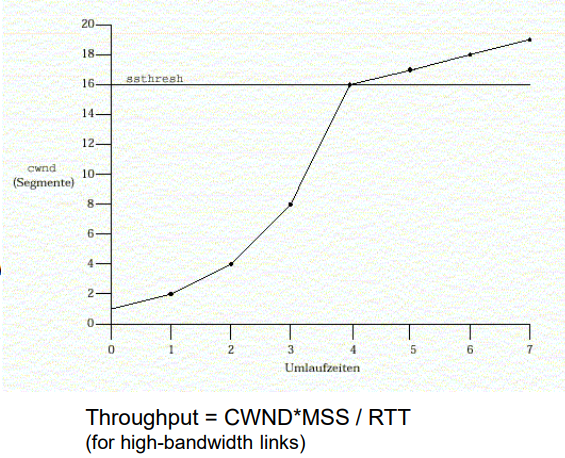
\includegraphics[width=\linewidth]{CWMD.png}
\end{minipage}\hfill
\begin{minipage}[t]{0.57\textwidth}
\vspace{0pt}
\begin{defbox}
\textbf{Start:} cwnd $= 1$ segment.\\[2pt]
\textbf{Slow Start} (exp.): cwnd $\times 2$ per RTT until ssthresh.\\[2pt]
\textbf{Congestion Avoidance} (linear): cwnd $+1$ per RTT.\\[2pt]
ssthresh init $\to$ user defined.
\end{defbox}
\vspace{2pt}
\begin{warnbox}
\textbf{Triple dup ACK} --- receiver keeps ACKing same seq.\ no., but later pkts \emph{are} arriving (out of order) $\Rightarrow$ one pkt missing, path still works. Fast Retransmit:\\
ssthresh $=$ cwnd$/2$,\quad restart at cwnd$/2$.\\[4pt]
\textbf{Timeout / RTO} --- RTO (est.\ from RTT) expires, no ACK at all $\Rightarrow$ neither pkts reaching dst nor ACKs returning, severe loss:\\
ssthresh $=$ cwnd$/2$,\quad cwnd $= 1$,\quad restart slow start.
\end{warnbox}
\end{minipage}
\textbf{We can conclude:}
TCP maximises throughput while avoiding congestion via a dynamic congestion window.

% ===========================================================================
\section*{1b\quad Flow Control \& Congestion Window Interaction \& (interaction with Layer 2 (WLAN))}
% ===========================================================================

Flow control (rwnd) and congestion control (cwnd) are \textbf{independent} limits --- both apply at all times, the sender is bounded by whichever is smaller:
\begin{keybox}
\textbf{Sliding window / rwnd} $\to$ protect \emph{receiver} buffer (set by receiver in each ACK)\\
\textbf{Congestion window / cwnd} $\to$ protect \emph{network} (set by sender via AIMD)\\
\textbf{Usable window} $= \min(\text{rwnd},\,\text{cwnd})$ \quad --- cwnd may grow past rwnd, but min caps actual sending
\end{keybox}

\vspace{2pt}

\begin{warnbox}
\small\textbf{L2 interaction (e.g.\ WLAN):} L2 protocols like 802.11 have their own \textbf{retransmissions} and \textbf{rate adaptation} (dropping from e.g.\ 54$\to$11\,Mbps on poor signal). Both happen invisibly below TCP.\\[2pt]
TCP never sees a packet loss $\Rightarrow$ cwnd never backs off $\Rightarrow$ cwnd keeps growing, until it hits the effective L2 throughput ceiling. \\[2pt] 
This effect is clearly observable: TCP throughput plateaus at the L2-adapted rate rather than the nominal link rate.
\end{warnbox}


\vspace{2pt}


\section{Note and Example (Only if they ask)}
\begin{notebox}
\vspace{0pt}
\begin{minipage}[c]{0.50\textwidth}
\vspace{0pt}
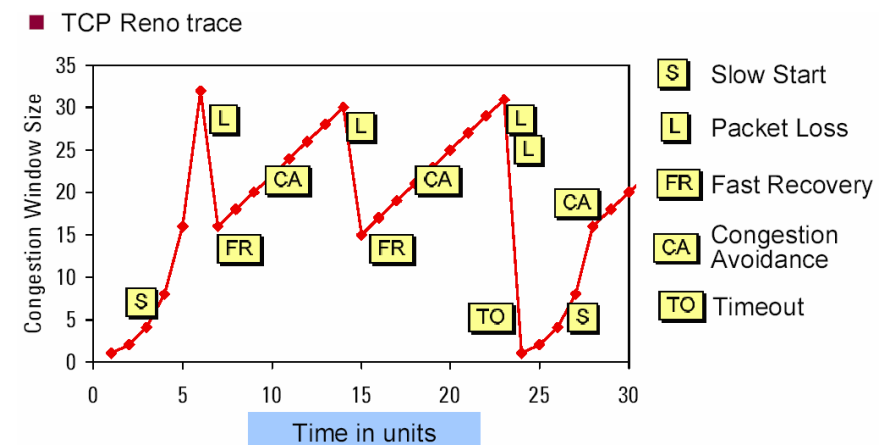
\includegraphics[width=\linewidth]{CWMDexample.png}
\end{minipage}\hfill
\begin{minipage}[c]{0.47\textwidth}
\vspace{0pt}
\textbf{TCP Reno trace:} 
\begin{itemize}
  \item S=Slow Start
  \item L=Loss
  \item FR=Fast Recovery, FR only halves --- much less disruptive.
  \item CA=Cong.\ Avoid
  \item TO=Timeout, TO resets cwnd$=1$;
\end{itemize}
\end{minipage}
\end{notebox}
\clearpage
% ===========================================================================
\section*{2\quad Fixpoint Model: TCP + Network Mutually Dependent}
% ===========================================================================

TCP and the network are \textbf{mutually dependent} --- each affects the other continuously:

\begin{keybox}
TCP sends faster $\Rightarrow$ network congests $\Rightarrow$ loss $p$ and delay $d$ increase $\Rightarrow$ TCP backs off $\Rightarrow$ congestion eases $\Rightarrow$ TCP speeds up again.\\[2pt]
They \textbf{co-determine} each other --- neither can be solved in isolation.
\end{keybox}

We model this with a \textbf{fixpoint model} (basically to get queue bottlenck/congestion): 
\begin{itemize}
  \item a feedback loop between a TCP model and a network model iterated until stable
  \item The diagram below is an interpretation of the expected interaction between the two.
\end{itemize}

\vspace{2pt}

\vspace{0pt}
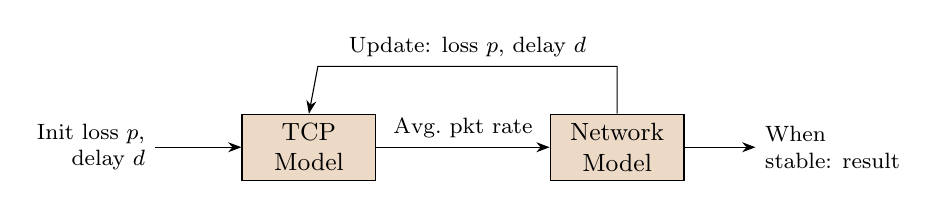
\begin{tikzpicture}[>=Stealth, font=\small, node distance=0.5cm]
  \node[draw, fill=brown!30, minimum width=1.7cm, minimum height=0.7cm, align=center] (tcp) {TCP\\Model};
  \node[draw, fill=brown!30, minimum width=1.7cm, minimum height=0.7cm, align=center, right=2.2cm of tcp] (net) {Network\\Model};
  \node[left=1.1cm of tcp, align=right, font=\footnotesize] (init) {Init loss $p$,\\delay $d$};
  \node[right=0.9cm of net, font=\footnotesize, align=left] (res) {When\\stable: result};
  \draw[->] (init) -- (tcp);
  \draw[->] (tcp) -- node[above, font=\footnotesize]{Avg.\ pkt rate} (net);
  \draw[->] (net) -- (res);
  \draw[->] (net.north) -- ++(0,0.6)
    -- node[above, font=\footnotesize]{Update: loss $p$, delay $d$}
    ++(-3.8,0) -- (tcp.north);
\end{tikzpicture}

\begin{keybox}
\small\textbf{TCP model} (Padhye et al.): analytical formula capturing slow start, cwnd dynamics and backoff --- takes loss $p$ and delay $d$ as input, outputs \textbf{throughput} $T$ (pkts/s).\\[4pt]
\textbf{Network model} (e.g.\ M/M/1/K): chosen to reflect expected network behaviour --- buffer overflow $\Rightarrow$ congestion, packet drops. Takes $T$ as arrival rate, returns updated $p$ and $d$.\\[4pt]
\textbf{Iteration:}
\begin{enumerate}
  \item Initialise with a guess for $p$, $d$
  \item TCP model $\to$ compute $T(p,d)$
  \item Network model $\to$ compute $p(T)$, $d(T)$
  \item Repeat until $p$, $d$, $T$ no longer change $\to$ \textbf{fixpoint reached}
\end{enumerate}
\end{keybox}
\vspace{2pt}
\begin{notebox}
\textbf{Padhye [Sigcomm 98]} (if asked) --- $T$ = throughput (pkts/s):
\[
T \!\approx\! \frac{1}{\overline{RTT}}\min\!\left(\!W_{\max},\,\frac{1}{\sqrt{\frac{2bp}{3}}+\frac{T_0}{\overline{RTT}}\min(1,3\sqrt{\frac{3bp}{8}})\,p(1{+}32p^2)}\right)
\]
\begin{itemize}
  \item $b$: number of packets acknowledged per ACK
  \item $\overline{RTT}$: average round-trip time (incl.\ queuing delay)
  \item $W_{\max}$: maximum congestion window size
  \item $T_0$: average timeout interval
  \item $p$: fraction of retransmitted packets (loss rate)
\end{itemize}
\end{notebox}

% ===========================================================================
\section*{3\quad Results: File Transfer Delays --- Model vs.\ Measurement}
% ===========================================================================

\vspace{0pt}
\begin{minipage}[t]{0.55\textwidth}
\vspace{0pt}
\includegraphics[page=25, width=\linewidth, trim=0 110 0 155, clip]{../../Slides/2026_MM6_TCP_Performance.pdf}
\end{minipage}\hfill
\begin{minipage}[t]{0.37\textwidth}
\vspace{0pt}
\begin{warnbox}
\small\textbf{Model deviates significantly.}\\[2pt]
At 9\% packet loss: TCP model $\approx500\,\text{ms}$, measured $\approx27000\,\text{ms}$ --- 50$\times$ error.\\[3pt]
Extended TCP model (adds bandwidth limits) tracks measured much better.\\[3pt]
Use fixpoint as estimate only.
\end{warnbox}
\end{minipage}

\vspace{3pt}

% ===========================================================================
\section*{4\quad Model 3: Multiple Connections --- Discouraged Arrivals}
% ===========================================================================

\vspace{0pt}
\begin{minipage}[t]{0.52\textwidth}
\vspace{0pt}
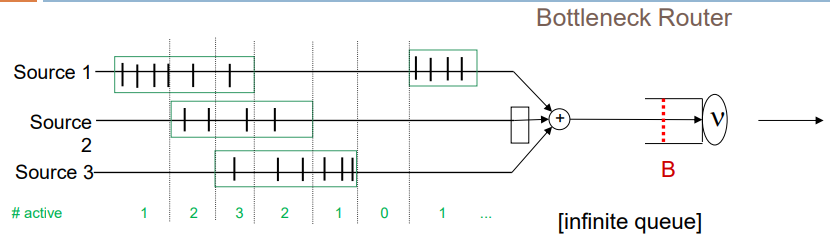
\includegraphics[width=\linewidth]{bottleneckSources.PNG}
\end{minipage}\hfill
\begin{minipage}[t]{0.45\textwidth}
\vspace{0pt}
\begin{keybox}
\small $j$ connections share bottleneck (rate $\nu$, buffer $B$).\\[2pt]
Rate per conn: $\lambda_p$ if $j\lambda_p \leq \nu$; else $\delta\nu/j$.\\[2pt]
\textbf{Why $\delta < 1$ (not 100\% util.):} TCP does slow start, backs off on every loss/timeout, and never runs at full rate --- it constantly probes and retreats. So actual throughput $\approx \delta \times$ ideal, with $\delta \leq 1$ derived from TCP loss behaviour.
\end{keybox}
\vspace{2pt}
\begin{notebox}
\small Congestion feedback $\to$ \textbf{Markov chain} (no closed form). Buffer fills before max TP is reached. Model 3 = ON/OFF arrivals with queue-dependent rate.
\end{notebox}
\end{minipage}

\vspace{4pt}
\clearpage
\section{Extra Shit i Cant take with Me into the Exam}
% ===========================================================================
\section*{5\quad Connection Level Model --- Why Analytically Better}
% ===========================================================================

\vspace{0pt}
\begin{minipage}[t]{0.48\textwidth}
\vspace{0pt}
\begin{keybox}
\small\textbf{What it does (Heyman et al.):} $N$ TCP sources share bottleneck rate $\nu$. Modified Processor Sharing (M/M/1//N/PS): $j$ active conns each get $\lambda_p$ if $j\lambda_p \leq \nu$, else $\delta\nu/j$. Yields \textbf{closed-form} stationary distribution --- no iteration.
\end{keybox}
\end{minipage}\hfill
\begin{minipage}[t]{0.48\textwidth}
\vspace{0pt}
\begin{notebox}
\small\textbf{vs.\ Model 3:} ON/OFF arrivals throttled by congestion $\Rightarrow$ Markov chain, no closed form, numerical only.\\[2pt]
\textbf{Why better:} direct analytical throughput distribution; captures connection arrival/departure dynamics; no heuristic fixpoint iteration required.
\end{notebox}
\end{minipage}

\vspace{4pt}

% ===========================================================================
\section*{6\quad TCP Handshake, Sequence Numbers \& Teardown}
% ===========================================================================

\vspace{0pt}
\begin{minipage}[t]{0.3\textwidth}
\vspace{0pt}
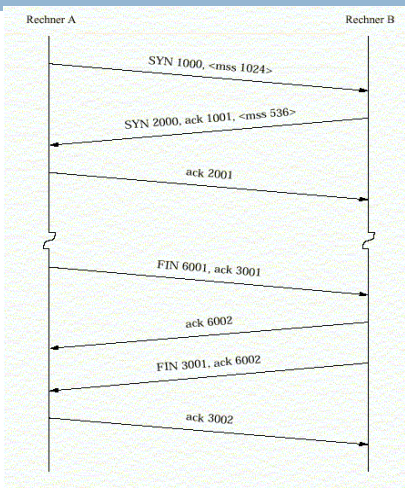
\includegraphics[width=\linewidth]{handshake.png}
\end{minipage}\hfill
\begin{minipage}[t]{0.60\textwidth}
\vspace{0pt}
\begin{keybox}
\small\textbf{3-Way Handshake:}
\begin{enumerate}
  \item \textbf{SYN}: Client $\to$ Server; seq$=x$, MSS option
  \item \textbf{SYN-ACK}: Server $\to$ Client; seq$=y$, ack$=x{+}1$, MSS option
  \item \textbf{ACK}: Client $\to$ Server; ack$=y{+}1$
\end{enumerate}
\textbf{Seq numbers} count \emph{bytes} sent (not packets) --- increments by bytes in each segment. \textbf{MSS} negotiated in SYN options; min of both sides is used.
\end{keybox}
\vspace{2pt}
\begin{notebox}
\small\textbf{FIN} (graceful): 4-way close --- FIN, ACK, FIN, ACK; each side closes independently (half-close). \textbf{RST}: immediate abort on error or connection refused.
\end{notebox}
\end{minipage}

\vspace{4pt}

% ===========================================================================
\section*{7\quad Flow Control vs.\ Congestion Control}
% ===========================================================================

\vspace{0pt}
\begin{minipage}[t]{0.57\textwidth}
\vspace{0pt}
\includegraphics[page=6, width=\linewidth, trim=0 20 0 55, clip]{../../Slides/2026_MM6_TCP_Performance.pdf}
\end{minipage}\hfill
\begin{minipage}[t]{0.40\textwidth}
\vspace{0pt}
\begin{defbox}
\small\textbf{Flow Control} (protects \emph{receiver}):\\[2pt]
Receiver advertises \textbf{rwnd} = offered window = free buffer space in ACKs. This sets the right edge of the window.\\[2pt]
\textbf{Sliding window:} left edge advances as ACKs arrive; right edge $= \min(\mathrm{cwnd},\,\mathrm{rwnd})$.
\end{defbox}
\vspace{2pt}
\begin{keybox}
\small\textbf{Congestion Control} (protects \emph{network}):\\[2pt]
\textbf{cwnd} probes for usable bandwidth (slow start, CA). Also limits right edge.\\[2pt]
\textbf{Usable window} = right-edge portion not yet sent (segments 7--9 in figure).
\end{keybox}
\end{minipage}



\end{document}
